\documentclass[12pt]{article}
\usepackage[margin=1in]{geometry}
\usepackage{enumitem}
\usepackage{caption}
\usepackage[subrefformat=parens,labelformat=parens]{subcaption}
\usepackage{graphicx}
\graphicspath{{figures/}}

\title{
  \vspace{-2cm}
  CSE 455 Homework 5 \\
  \author{Yoshihiro Kumazawa}
}

\begin{document}
\maketitle

\section{Installing PyTorch}
Done!

\section{Find the best network}
\subsection{Training a classifier using only one fully connected Layer}
See Figure~\ref{fig:2_1}. We can say that the the model successfully trained since the loss is decreasing throughout the training process and there is a healthy gap between the training accuracy and testing accuracy.

\subsection{Training a classifier using multiple fully connected Layers}
See Figure~\ref{fig:2_2}. The training is not successful because the testing accuracy plateaus whereas the training keeps increasing.

\subsubsection{Question}
See Figure~\ref{fig:2_2_1}. The model accuracy is significantly worse than the previous model. This is because the model is expressively limited since it has less non-linearity. The model can actually become just as good as LazyNet since without activations, the forward pass is just a couple of matrix multiplications, which is nothing but a single matrix multiplication by the composed matrices. But somehow, by separating the weight update process in back propagation, it achieves a slightly higher accuracy than LazyNet.

\begin{figure}
  \begin{subfigure}{0.16\textwidth}
    \centering
    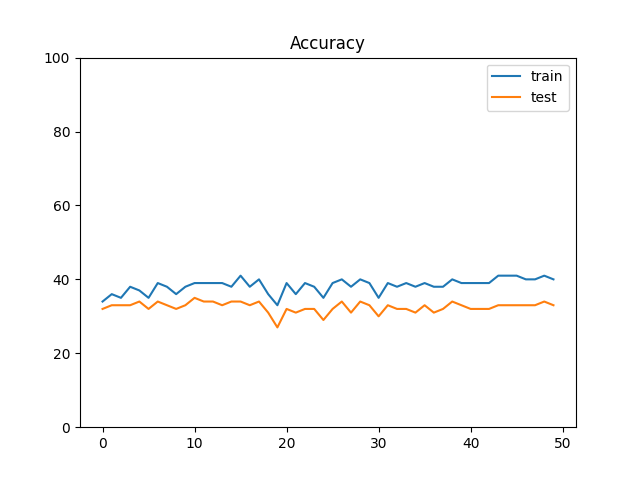
\includegraphics[width=\linewidth]{accuracies_2_1.png}
  \end{subfigure}
  \begin{subfigure}{0.16\textwidth}
    \centering
    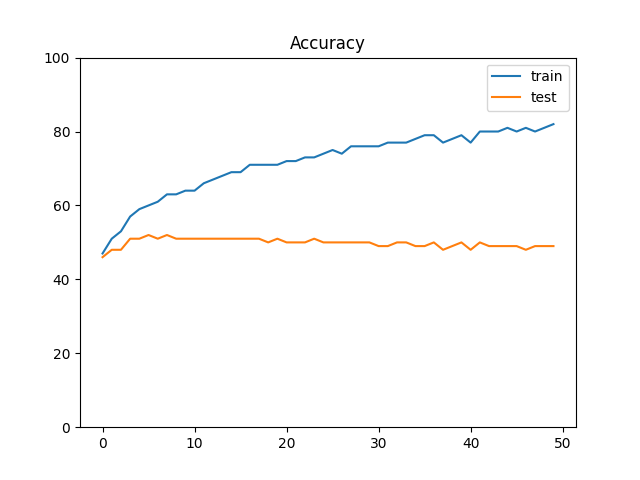
\includegraphics[width=\linewidth]{accuracies_2_2.png}
  \end{subfigure}
  \begin{subfigure}{0.16\textwidth}
    \centering
    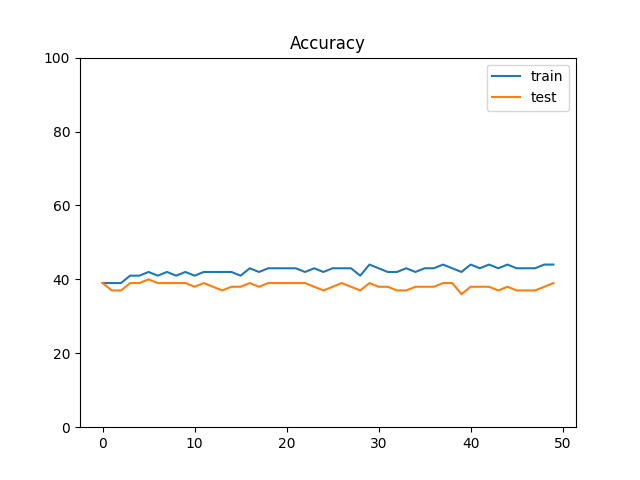
\includegraphics[width=\linewidth]{accuracies_2_2_1.png}
  \end{subfigure}

  \begin{subfigure}{0.16\textwidth}
    \centering
    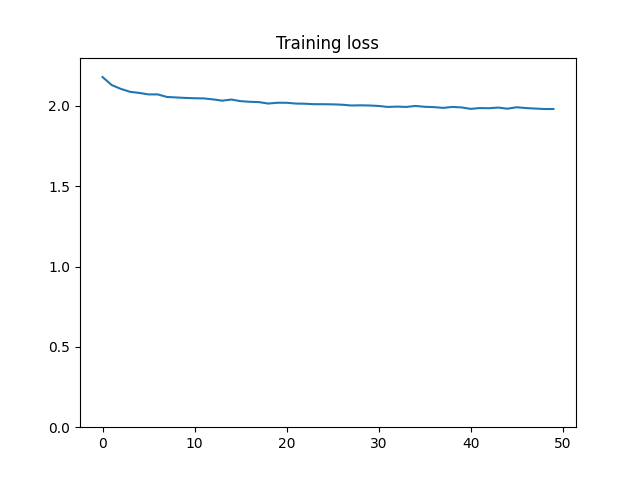
\includegraphics[width=\linewidth]{loss_2_1.png}
    \caption{}
    \label{fig:2_1}
  \end{subfigure}
  \begin{subfigure}{0.16\textwidth}
    \centering
    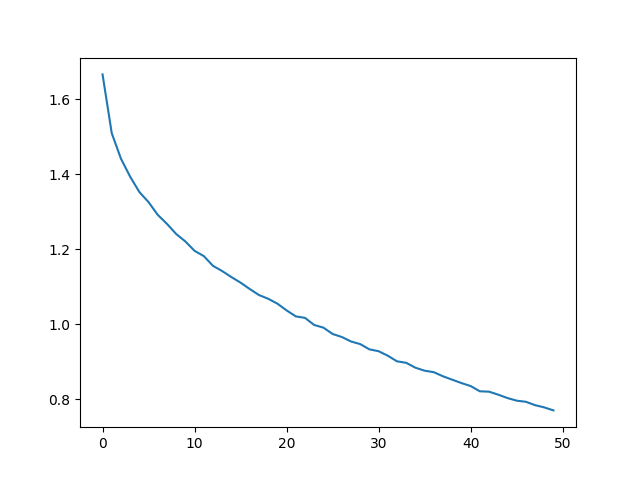
\includegraphics[width=\linewidth]{loss_2_2.png}
    \caption{}
    \label{fig:2_2}
  \end{subfigure}
  \begin{subfigure}{0.16\textwidth}
    \centering
    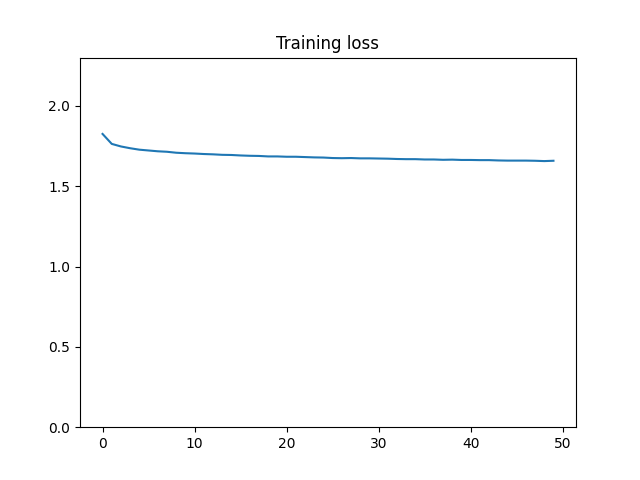
\includegraphics[width=\linewidth]{loss_2_2_1.png}
    \caption{}
    \label{fig:2_2_1}
  \end{subfigure}
  \caption{Training results of LazyNet and BoringNet: \subref{fig:2_1} LazyNet, \subref{fig:2_2} BoringNet, \subref{fig:2_2_1} BoringNet without activations.}
  \label{fig:images}
\end{figure}

\subsection{Training a classifier using convolutions}
\subsubsection{Question}

\section{How does learning rate work?}

\section{Data Augmentation}

\section{Change the loss function}

\end{document}
